\section{Letter to the Chief Operations Officer of HiMCM}

Dear Chief Operations Officer,

\indent Our investigation of six bus and rail waiting areas across Boston, Dallas, and Phoenix revealed an important finding: more cooling does not always mean better cooling. For Boston's Grove Hall bus shelter, we recommend a three-stage strategy: leave cooling off when conditions are comfortable, use a low-energy fan as the primary source of relief, and reserve the larger evaporative cooler for periods requiring stronger cooling. By adapting to passenger conditions rather than operating continuously, Grove Hall can balance comfort, sustainability, and cost.

\indent To develop this strategy, we compared three systems—a fan, a standard evaporative cooler, and a larger evaporative cooler—alongside no cooling, under peak-temperature, hot-humid, and hot-dry conditions from summer 2025. We evaluated comfort using Standard Effective Temperature (SET), which accounts for temperature, humidity, airflow, and other influences on perceived heat. Our model compares each system's ability to achieve a target range of 23–26°C SET against its electricity consumption, water use, and cost.

\indent Our first recommendation is to make the fan Grove Hall's primary cooling system. Under hot-humid conditions, the fan reduces predicted SET from 27.66°C to 25.09°C, bringing passengers within our comfort range. Both evaporative coolers also achieve this, but the fan consumes 90\% less electricity than the larger cooler and saves approximately 44 kg of water per hour. Its reference purchase price of \$1,499 is also considerably lower than the \$4,159 and \$4,939 alternatives~\cite{aireye_20_price,portacool_2000,portacool_4000}. Thus, when the fan provides sufficient relief, stronger cooling offers little additional benefit to justify its resource demands.

\indent During peak heat, however, stronger cooling becomes more valuable. The larger cooler reduces predicted SET from 30.77°C to 28.57°C, compared with 29.07°C for the fan. Our minimax-regret model consequently favors the larger cooler for minimizing worst-case discomfort across the three scenarios. Yet this additional half-degree of relief requires ten times the electricity and approximately 81 kg of evaporated water per hour. We therefore recommend reserving it for periods when the fan cannot provide adequate relief, rather than using it as the default system.

\indent Equally important is knowing when not to cool. Under Boston's hot-dry scenario, the uncooled shelter already achieves 24.44°C SET, within our target range, while all three active systems lower SET below it. We therefore recommend turning equipment off when conditions are already comfortable, avoiding unnecessary electricity and water consumption.

\indent Nevertheless, even the largest cooler cannot achieve our comfort target during peak heat. Grove Hall should therefore supplement its cooling systems with clear passenger guidance and access to air-conditioned refuge during hazardous conditions. Our comfort range is not a safety threshold, and passenger safety must always take precedence over resource efficiency.

\indent Overall, we recommend that Grove Hall adopt this condition-dependent strategy, prioritizing the fan's substantial energy and cost advantages while retaining stronger cooling for periods of greatest need. Our findings suggest that efficient cooling is not about using the most powerful equipment, but about delivering the right amount of relief to the people who need it, when they need it.

\indent We have also attached a blog post on the next page of this letter to expound on our results to the public.

Yours sincerely,

Team 19678

\begin{figure}[H]
    \centering
    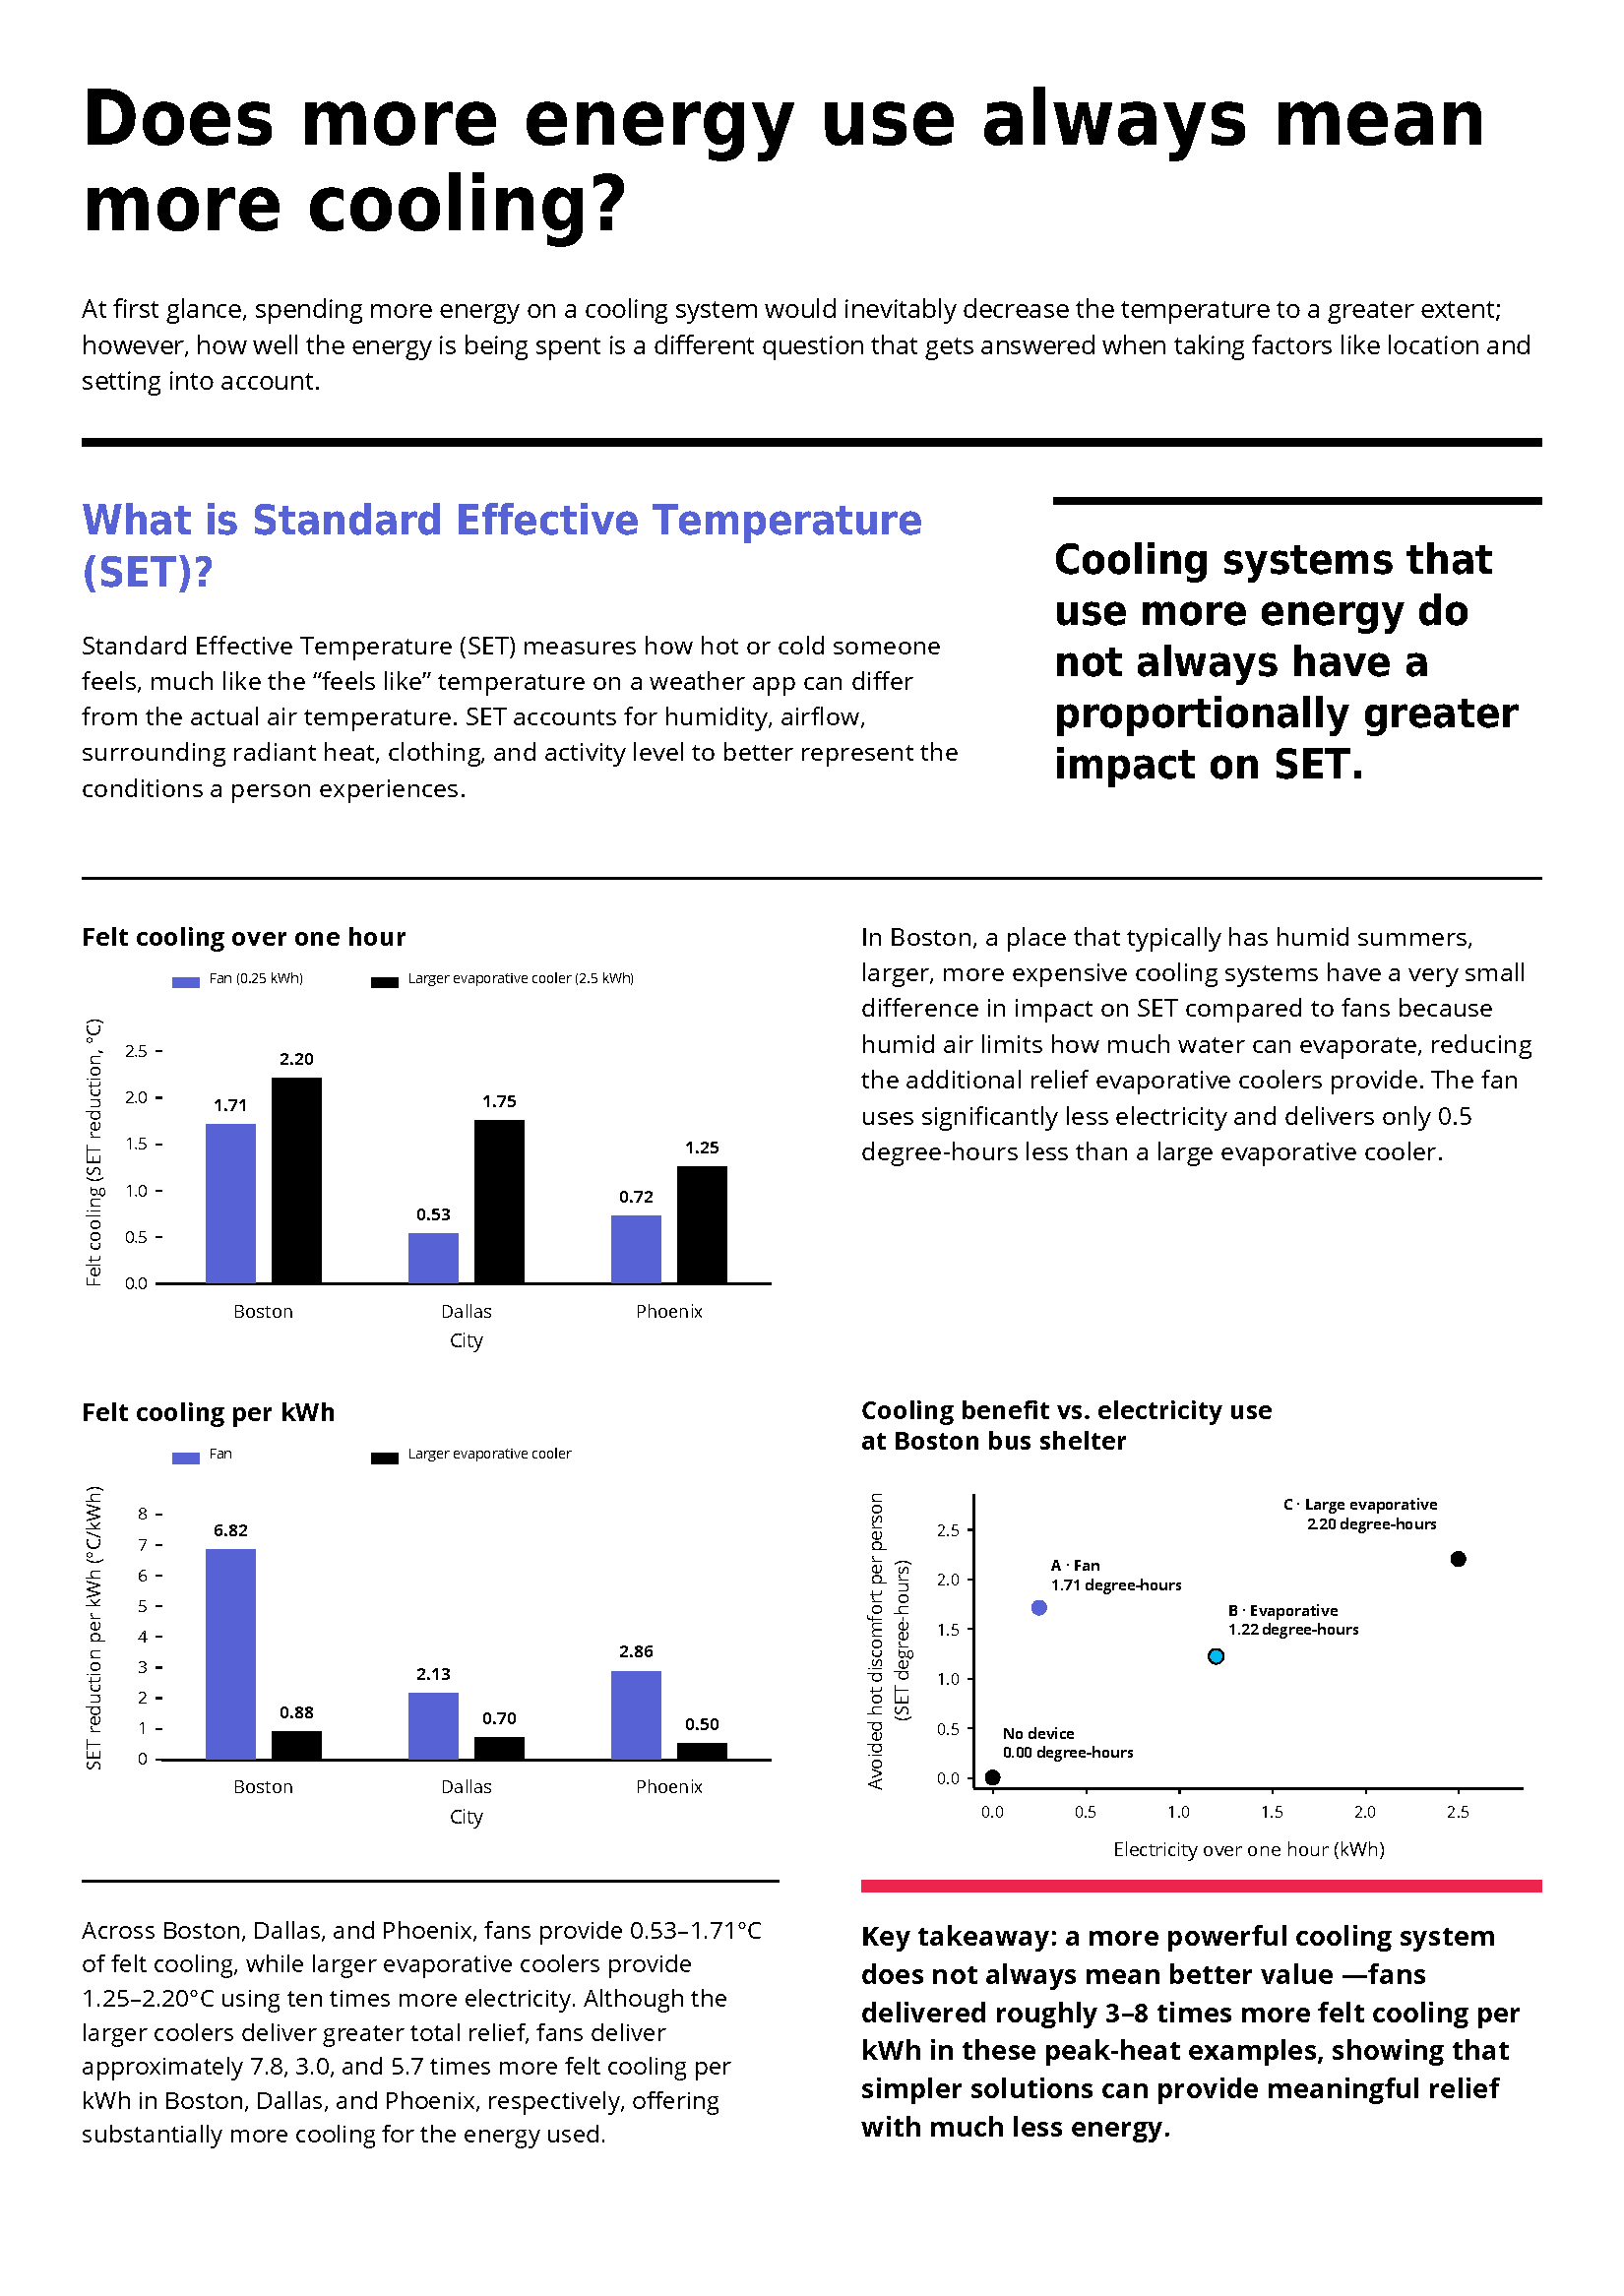
\includegraphics[width=0.88\linewidth]{Images/HiMCM26_BlogPost_Designed.pdf}
    \label{fig:blog-post}
\end{figure}